\documentclass[noauthor,nooutcomes,handout]{ximera}

\graphicspath{  
{./}
{./whoAreYou/}
{./drawingWithTheTurtle/}
{./bisectionMethod/}
{./circles/}
{./anglesAndRightTriangles/}
{./lawOfSines/}
{./lawOfCosines/}
{./plotter/}
{./staircases/}
{./pitch/}
{./qualityControl/}
{./symmetry/}
{./nGonBlock/}
}


%% page layout
\usepackage[cm,headings]{fullpage}
\raggedright
\setlength\headheight{13.6pt}


%% fonts
\usepackage{euler}

\usepackage{FiraMono}
\renewcommand\familydefault{\ttdefault} 
\usepackage[defaultmathsizes]{mathastext}
\usepackage[htt]{hyphenat}

\usepackage[T1]{fontenc}
\usepackage[scaled=1]{FiraSans}

%\usepackage{wedn}
\usepackage{pbsi} %% Answer font


\usepackage{cancel} %% strike through in pitch/pitch.tex


%% \usepackage{ulem} %% 
%% \renewcommand{\ULthickness}{2pt}% changes underline thickness

\tikzset{>=stealth}

\usepackage{adjustbox}

\setcounter{titlenumber}{-1}

%% journal style
\makeatletter
\newcommand\journalstyle{%
  \def\activitystyle{activity-chapter}
  \def\maketitle{%
    \addtocounter{titlenumber}{1}%
                {\flushleft\small\sffamily\bfseries\@pretitle\par\vspace{-1.5em}}%
                {\flushleft\LARGE\sffamily\bfseries\thetitlenumber\hspace{1em}\@title \par }%
                {\vskip .6em\noindent\textit\theabstract\setcounter{question}{0}\setcounter{sectiontitlenumber}{0}}%
                    \par\vspace{2em}
                    \phantomsection\addcontentsline{toc}{section}{\thetitlenumber\hspace{1em}\textbf{\@title}}%
                     }}
\makeatother



%% thm like environments
\let\question\relax
\let\endquestion\relax

\newtheoremstyle{QuestionStyle}{\topsep}{\topsep}%%% space between body and thm
		{}                      %%% Thm body font
		{}                              %%% Indent amount (empty = no indent)
		{\bfseries}            %%% Thm head font
		{)}                              %%% Punctuation after thm head
		{ }                           %%% Space after thm head
		{\thmnumber{#2}\thmnote{ \bfseries(#3)}}%%% Thm head spec
\theoremstyle{QuestionStyle}
\newtheorem{question}{}



\let\freeResponse\relax
\let\endfreeResponse\relax

%% \newtheoremstyle{ResponseStyle}{\topsep}{\topsep}%%% space between body and thm
%% 		{\wedn\bfseries}                      %%% Thm body font
%% 		{}                              %%% Indent amount (empty = no indent)
%% 		{\wedn\bfseries}            %%% Thm head font
%% 		{}                              %%% Punctuation after thm head
%% 		{3ex}                           %%% Space after thm head
%% 		{\underline{\underline{\thmname{#1}}}}%%% Thm head spec
%% \theoremstyle{ResponseStyle}

\usepackage[tikz]{mdframed}
\mdfdefinestyle{ResponseStyle}{leftmargin=1cm,linecolor=black,roundcorner=5pt,
, font=\bsifamily,}%font=\wedn\bfseries\upshape,}


\ifhandout
\NewEnviron{freeResponse}{}
\else
%\newtheorem{freeResponse}{Response:}
\newenvironment{freeResponse}{\begin{mdframed}[style=ResponseStyle]}{\end{mdframed}}
\fi



%% attempting to automate outcomes.

%% \newwrite\outcomefile
%%   \immediate\openout\outcomefile=\jobname.oc
%% \renewcommand{\outcome}[1]{\edef\theoutcomes{\theoutcomes #1~}%
%% \immediate\write\outcomefile{\unexpanded{\outcome}{#1}}}

%% \newcommand{\outcomelist}{\begin{itemize}\theoutcomes\end{itemize}}

%% \NewEnviron{listOutcomes}{\small\sffamily
%% After answering the following questions, students should be able to:
%% \begin{itemize}
%% \BODY
%% \end{itemize}
%% }
\usepackage[tikz]{mdframed}
\mdfdefinestyle{OutcomeStyle}{leftmargin=2cm,rightmargin=2cm,linecolor=black,roundcorner=5pt,
, font=\small\sffamily,}%font=\wedn\bfseries\upshape,}
\newenvironment{listOutcomes}{\begin{mdframed}[style=OutcomeStyle]After answering the following questions, students should be able to:\begin{itemize}}{\end{itemize}\end{mdframed}}



%% my commands

\newcommand{\snap}{{\bfseries\itshape\textsf{Snap!}}}
\newcommand{\flavor}{\link[\snap]{https://snap.berkeley.edu/}}
\newcommand{\mooculus}{\textsf{\textbf{MOOC}\textnormal{\textsf{ULUS}}}}


\usepackage{tkz-euclide}
\tikzstyle geometryDiagrams=[rounded corners=.5pt,ultra thick,color=black]
\colorlet{penColor}{black} % Color of a curve in a plot



\ifhandout\newcommand{\mynewpage}{\newpage}\else\newcommand{\mynewpage}{}\fi


\title{The good Earth}
\author{Bart Snapp}

%% ONLY REQUIRES WHAT's YOUR ANGLE...



\begin{document}
\begin{abstract}
  We'll compute the circumference of the Earth.
\end{abstract}
\maketitle

\begin{listOutcomes}
\item Translate classroom mathematics into real world mathematics. 
\item Measure angles with a protractor.
\item Apply basic facts to solve for angles.
%\item Critique and dismantle reasonable hypotheses in regard to geometry and arithmetic.
\item Describe the historical methods for computing the circumference
    of the Earth.
\end{listOutcomes}
%


  Around $100$ BCE, \link[Eratosthenes of Cyrene]{https://en.wikipedia.org/wiki/Eratosthenes} read something very interesting:
  \begin{quote}
    At (solar) noon on the longest day of summer, in the ancient city of Syene
    (modern day \link[Aswan]{https://en.wikipedia.org/wiki/Aswan}) the
    Sun shines to the bottom of all open wells.
  \end{quote}
  He realized that this means
  that at noon, on the longest day, the Sun was directly overhead
  Aswan. Eratosthenes wondered if the Sun was also directly overhead
  \link[Alexandria]{https://en.wikipedia.org/wiki/Alexandria} on that
  same day. So, he put a stick perpendicularly into the ground, and
  saw that Sun was not directly overhead Alexandria at this time by
  observing the shadow of the stick. Eratosthenes was able to use this
  information, and a little more, to compute the circumference of the
  Earth. Wow!



  Now, you will play the role of Eratosthenes!
  \mynewpage
\begin{question}
Here is a schematic diagram of the situation:
    \begin{center}
      \begin{tikzpicture}[geometryDiagrams,scale=1.5]
        
        \coordinate (O) at (0,0);
        \coordinate (S) at (5,0);
        \coordinate (A) at (4.33,2.5);
        \coordinate (A') at (-4.33,-2.5);
        \coordinate (S') at (-5,0);
        \coordinate (K) at (5.16,3);
        \coordinate (KK) at (6.45,3.75);
        \coordinate (H) at (4.01,2.99);
        \coordinate (tsun1) at (10,2.99);
        \coordinate (tsun2) at (4.1,2.99);
        \coordinate (bsun1) at (10,0);
        \coordinate (bsun2) at (5,0);
        
        \begin{scope}
        \clip (-1,-1) rectangle (6,4);
        \tkzDrawCircle[fill=blue!10!white,draw=blue!50!black](O,A)
        \tkzDrawSegment[dashed](S',S)
        \tkzDrawSegment[dashed](A',KK)
        \tkzDrawSegment[line width=1mm, black,line cap=rect](A,H)
        \tkzDrawSegment[line width=1mm, black!20!brown](K,A)
        \end{scope}
        \tkzDrawSegment[line width=1mm, yellow!50!orange,->](tsun1,tsun2)
        \tkzDrawSegment[line width=1mm, yellow!50!orange,->](bsun1,bsun2)

        \node at (8.5,1.5) {Sun's rays};

        \node at (5.2,2.7) {stick};

        \node at (3.6,2.7) {shadow};
        \tkzDrawPoint(O)
        \tkzDrawPoint(A)
        \tkzDrawPoint(S)

        \node at (5.2,2.4) {Alexandria};
        \node at (5.5,-.3) {Aswan};
        
        \node at (1,-.3) {center of the Earth};

        \node at (4.7,2.87) {$\alpha$};

        \node at (.6,.15) {$\beta$};

        \tkzMarkAngle[size=.5,mark={}](S,O,A)

        \tkzMarkAngle[size=.3,mark={}](H,K,A)
      \end{tikzpicture}
    \end{center}
    Explain why:
    \begin{enumerate}
    \item The Sun's rays are essentially parallel.
    \item The angle opposite $\alpha$ has the same measure as $\beta$.
    \item The the measure of angle $\alpha$ is the same as the measure
      of angle $\beta$. If you use a famous theorem, you need to
      explain why that is true too.
    \end{enumerate}
\end{question}










\mynewpage




\begin{question}
  Here is an accurate (up-to-scale) drawing of the stick and the
  shadow at Alexandria, during the longest day of summer at noon.
  Identify and measure the relevant angle(s):
    %% 7.2 degrees 
    \begin{center}
        \begin{tikzpicture}[geometryDiagrams,scale=3]
        \coordinate (O) at (0,0); \coordinate (T) at (0,6);
        \coordinate (S) at (-.75,0); \tkzDrawSegment[line
          width=2mm,black](O,S) \tkzDrawSegment[line width=2mm,
          black!20!brown,line cap=rect](O,T)
        \end{tikzpicture}
    \end{center}

 \end{question}
 \mynewpage

\begin{question}
Eratosthenes had someone ``pace'' the distance from Alexandria
    to Aswan, and found it to be around $500$ miles. 
\begin{enumerate}
 \item Use this new information, along with the previous problems, to
   estimate the circumference of the Earth.
 \item Now let's think critically about some fun facts!
   \begin{description}
   \item[Fun fact 1:] The actual circumference of the Earth at the
     equator is $24,901$ miles.
   \item[Fun fact 2:] The actual latitude of Alexandria is 31.2
     degrees North and the actual latitude of Aswan is 24.1 degrees
     North. The distance between them 524 miles. If we use
     Eratosthenes' method with these \textbf{correct} numbers, we find
     the circumference of the Earth to be $26,569$ miles.
   \end{description}
   How is it possible that this computation is wrong (it's too large)?
   \begin{hint}
     Look at a map.
   \end{hint}
\end{enumerate}

 \end{question}

\end{document}

%  \begin{freeResponse}
%    \begin{enumerate}
%      \item The Sun's rays are approximately parallel when they hit
%        the Earth because the Sun is so incredibly far from the
%        Earth. You can DIRECTLY OBSERVE this fact if you ever notice
%        that the Sun seems to follow you as you travel.
%      \item I'll reproduce the diagram here with one more angle marked:
%        \begin{center}
%          \begin{tikzpicture}[geometryDiagrams,scale=1.5]
%            
%            \coordinate (O) at (0,0);
%            \coordinate (S) at (5,0);
%            \coordinate (A) at (4.33,2.5);
%            \coordinate (A') at (-4.33,-2.5);
%            \coordinate (S') at (-5,0);
%            \coordinate (K) at (5.16,3);
%            \coordinate (KK) at (6.45,3.75);
%            \coordinate (H) at (4.01,2.99);
%            \coordinate (tsun1) at (10,2.99);
%            \coordinate (tsun2) at (4.1,2.99);
%            \coordinate (bsun1) at (10,0);
%            \coordinate (bsun2) at (5,0);
%            
%            \begin{scope}
%              \clip (-1,-1) rectangle (6,4);
%              \tkzDrawCircle[fill=blue!10!white,draw=blue!50!black](O,A)
%              \tkzDrawSegment[dashed](S',S)
%              \tkzDrawSegment[dashed](A',KK)
%              \tkzDrawSegment[line width=1mm, black,line cap=rect](A,H)
%              \tkzDrawSegment[line width=1mm, black!20!brown](K,A)
%            \end{scope}
%            \tkzDrawSegment[line width=1mm, yellow!50!orange,->](tsun1,tsun2)
%            \tkzDrawSegment[line width=1mm, yellow!50!orange,->](bsun1,bsun2)
%            
%            \node at (8.5,1.5) {Sun's rays};
%
%            \node at (5.2,2.7) {stick};
%            
%            \node at (3.6,2.7) {shadow};
%            \tkzDrawPoint(O)
%            \tkzDrawPoint(A)
%            \tkzDrawPoint(S)
%            
%            \node at (5.2,2.4) {Alexandria};
%            \node at (5.5,-.3) {Aswan};
%            
%            \node at (1,-.3) {center of the Earth};
%            
%            \node at (4.7,2.87) {$\alpha$};
%            
%            \node at (.6,.15) {$\beta$};
%            \node at (5.8,3.15) {$\gamma$};
%            
%            \tkzMarkAngle[size=.5,mark={}](S,O,A)
%            \tkzMarkAngle[size=.5,mark={}](tsun1,K,KK)
%        
%            \tkzMarkAngle[size=.3,mark={}](H,K,A)
%          \end{tikzpicture}
%        \end{center}
%        Since the Sun's rays are parallel, we see
%            $\beta=\gamma$. Since $\alpha$ and $\beta$ are vertical
%        angles, we see from ``What's Your Angle'' that $\gamma =
%        \alpha$, and hence $\alpha = \beta$.
%      \item I measured the angle with GeoGebra
%        \begin{center}
%          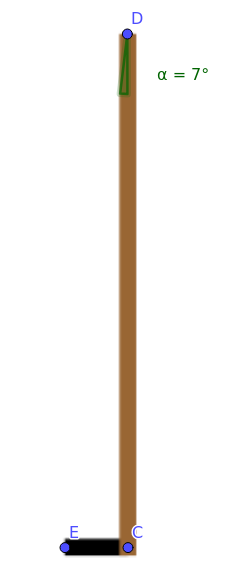
\includegraphics[width=.2\textwidth]{shadowFax.png}
%        \end{center}
%        From this we see the angle is around $7$ degrees.
%      \item The distance from Alexandria to Aswan is around $500$
%        miles, so
%        \[
%        \frac{360}{7}\cdot 500 \approx 25714~\text{miles}
%        \]
%        so the the Earth has about a $25000$ mile circumference. This is quite close to the current answer of $24901$ miles.
%      \item You don't need a clock, Eratosthenes surely just looked to
%        see when the shadow was SHORTEST. Since the Sun is highest at
%        noon, the shadow would be shortest at this time.
%        \end{enumerate}
%  \end{freeResponse}
%\end{question}
%\mynewpage
%
%\end{document}
%
%\begin{question}
%  Humans have known that the Earth was roughly spherical since the the
%  $5$th century BCE. In the argument above, Eratosthenes ASSUMES that
%  the Earth is spherical.
%\begin{quote}
%  Let us wonder, what if he didn't assume that the Earth was spherical?
%\end{quote}
%
%  If Eratosthenes had assumed a flat Earth, his schematic diagram
%  would look something like this:
%  \begin{center}
%      \begin{tikzpicture}[geometryDiagrams,scale=1.5]
%        
%        \coordinate (B1) at (-3,-2);
%        \coordinate (B2) at (3,-2);
%        \coordinate (E1) at (-5,0);
%        \coordinate (E2) at (5,0);
%        \coordinate (S) at (0,0);
%        \coordinate (A) at (2.5,0);
%        \coordinate (sun) at (0,3);
%        \coordinate (ts) at (2.5,.58);
%        \coordinate (es) at (3,0);
%        \coordinate (dsr) at (.2,2.85);
%        \coordinate (osr) at (0,2.75);
%        \coordinate (ab) at (0,.1);
%        
%        
%        \begin{scope}
%        \clip (-4,-1) rectangle (4,4);
%        \tkzDrawPolygon[fill=blue!10!white,draw=blue!50!black](B1,B2,E2,E1)
%        \end{scope}
%        
%        \tkzDrawSegment[line width=1mm, yellow!50!orange,->](dsr,ts)
%        \tkzDrawSegment[line width=1mm, yellow!50!orange,->](osr,ab)
%        
%        \node at (0,3.5) {Sun};
%        \node at (2.5,-.5) {Alexandria};
%        \node at (0,-.5) {Aswan};
%        \tkzDrawSegment[line width=1mm, black,line cap=rect](A,es)
%         \tkzDrawSegment[line width=1mm, black!20!brown](A,ts)
%        \tkzDrawPoint(A)
%         \tkzDrawPoint(S)
%         \tkzDrawPoint[yellow!50!orange,size=15](sun)
%         
%         
%
%
%         
%        %% \node at (.6,.15) {$\beta$};
%
%        %% \tkzMarkAngle[size=.5,mark={}](S,O,A)
%
%        %% \tkzMarkAngle[size=.3,mark={}](H,K,A)
%      \end{tikzpicture}
%  \end{center}
%  \begin{enumerate}
%  \item With these assumptions, how far would Eratosthenes deduce the
%    Sun is from the Earth?
%  \item The \textit{Tropic of Cancer} and the \textit{Tropic of
%    Capricorn} are around $3200$ miles apart. They are also, each
%    $23.5$ degrees from the equator.  Find the distance on a flat
%    Earth between the Tropics. Explain how this is verifiably WRONG.
%  \item \textit{Geometry Giorgio} has been quietly thinking. He suddenly
%  exclaimed
%  \begin{quote}
%    We KNOW the ACTUAL angle Eratosthenes's should have measured. We
%    KNOW the ACTUAL distance (as the plane flys), and we can see if
%    his idea was correct!
%  \end{quote}
%  Soon \textit{Geometry Giorgio} looks rather glum. When asked why,
%  says
%  \begin{quote}
%    I'm getting the WRONG answer, the numbers are much too LARGE!
%  \end{quote}
%  \textit{Geometry Giorgio's} has \textbf{correctly followed Eratosthenes
%  method,} and \textit{Geometry Giorgio} is \text{correct} to point out that
%  the \textbf{computation is MUCH too large} (when compared to the ACTUAL
%  circumference of the Earth) \textbf{for computational comfort.}
%
%  EXPLAIN how is it possible that \textit{Geometry Giorgio's}
%  computation is compatible with the known circumference of the Earth.
%  \end{enumerate}
%  \begin{freeResponse}
%    \begin{enumerate}
%      \item If he assumed a flat Earth, he must suppose that the Sun
%        is around $4000$ miles away.
%      \item In on a flat Earth, the distance between the equator and
%        the Tropics is around $1700$ miles, doubling we find this is
%        $3400$ miles, $200$ miles too large.
%      \item The number is too large because Aswan is not at the same
%        longitude as Alexandria.
%    \end{enumerate}
%  \end{freeResponse}
%\end{question}
%\mynewpage
%%
%%
%%
%%\begin{question}%%https://en.wikipedia.org/wiki/String_girdling_Earth 
%%  Here a problem that is at least $300$ years old, so let's call it an
%%  ``oldie, but a goodie!''
%%  \begin{quote}
%%    Imagine a chain, pulled tight around the Earth's equator. Suppose
%%    you add an extra $10'$ to the chain. The chain is then raised up
%%    UNIFORMLY, all around the Earth, as high as possible. How high is
%%    that?
%%  \end{quote}
%%  Supposing that
%%  \begin{itemize}
%%  \item There are $5280$ feet in a mile, and
%%  \item the radius of the Earth is $4000$ miles,
%%  \end{itemize}
%%  it is now time for YOU to try YOUR hand at this classic.
%%  \begin{enumerate}
%%  \item Give a solution based on FORMULAS. Show all work and express
%%    your answer in FEET.
%%  \item Give a solution based on SCALING. Show all work and express
%%    your answer in FEET.
%%  \item Is the answer surprising? YES or NO. EXPLAIN why you say YES or
%%    NO.
%%  \end{enumerate}
%%  \begin{freeResponse}
%%    \begin{enumerate}
%%    \item Let $h$ be the maximum height above the Earth to which we
%%      can uniformly raise the chain. Using formulas I find:
%%      \[
%%      2\pi(4000 + h) = 2\pi 4000 + 10/5280
%%      \]
%%      Solving for $h$ and converting to feet will solve the
%%      problem. Write:
%%      \begin{align*}
%%        2\pi(4000 + h) &= 8000\pi + 10/5280 \\
%%        8000\pi + 2\pi h &= 8000\pi + 10/5280\\
%%        2\pi h &= 10/5280\\
%%        h &= \frac{10}{2\pi \cdot 5280}~\text{miles}.
%%      \end{align*}
%%      This is
%%      \[
%%      \frac{10}{2\pi}\approx 1.6~\text{feet}.
%%      \]
%%    \item We are scaling the circumference by a factor of
%%      \[
%%      \frac{2\pi 4000 + 10/5280}{2\pi 4000}.
%%      \]
%%      Thus we are scaling the radius by THE SAME FACTOR. The scaled
%%      radius will be
%%      \begin{align*}
%%        \frac{2\pi 4000 + 10/5280}{2\pi 4000}\cdot 4000 &= \frac{2\pi 4000 + 10/5280}{2\pi}\\
%%        &=  4000 +  \frac{10}{2\pi5280}.
%%      \end{align*}
%%      So an increase of $\frac{10}{2\pi5280}$ miles. This is
%%      \[
%%      \frac{10}{2\pi}\approx 1.6~\text{feet}.
%%      \]
%%      
%%    \item Well, we are scaling the diameter by a small amount when
%%      compared to the Earth's circumference. Since
%%      \[
%%      \text{Earth's radius} < \text{Earth's circumference}
%%      \]
%%      we should expect less of a ``result'' from scaling the
%%      radius---so an answer between $0$ and $10$. So NO, I am not
%%      surprised.
%%    \end{enumerate}
%%    \end{freeResponse}
%%    \end{question}
%
%\end{document}
